%%
%% ****** ljmsamp.tex 13.06.2018 ******
%%
\documentclass[
11pt,%
tightenlines,%
twoside,%
onecolumn,%
nofloats,%
nobibnotes,%
nofootinbib,%
superscriptaddress,%
noshowpacs,%
centertags]%
{revtex4}
\usepackage{ljm}

\begin{document}
	
	
	\titlerunning{Short form of the title} % for running heads
	\authorrunning{V. P. Kosyakov} % for running heads
	%\authorrunning{First-Author, Second-Author} % for running heads
	
	\title{Investigation of the influence of weight coefficients in solving the problem of identification of permeability for an oil field}
	% Splitting into lines is performed by the command \\
	% The title is written in accordance with the rules of capitalization.
	
	\author{\firstname{V.~P.}~\surname{Kosyakov}}
	\email[E-mail: ]{lik.24@yandex.ru}
	\affiliation{Tyumen Branch of Khristianovich Institute of Theoretical and Applied Mechanics SB RAS, Taymirskaya Str. 74, 625026, Tyumen, Russia}
	
	
	\received{March 23, 2023} % The date of receipt to the editor, i.e. December 06, 2017
	
	\maketitle
	\textbf{Abstract}. In the process of modeling the development of an oil field, one of the important steps is the solution of the inverse problem, the solution of which, as a rule, consists in the selection of model parameters for the best fit to the history of development. To solve the inverse problem, heterogeneous initial data are used, the degree of influence on the result of the solution of which is determined by their weight coefficients. In addition, the purpose of modeling is not only to repeat the development indicators for the historical period, but also to obtain a reliable forecast of the behavior of the modeled object in the future.
	In this work, using the example of solving the problem of parametric identification of the permeability field for modeling the development of an oil field, a study was made of the influence of the choice of weight coefficients on the accuracy of the model tuning and its predictive characteristics. It is shown that the correct choice of weight coefficients makes it possible to obtain a model with the best predictive properties. To assess the accuracy of the model and select the option of its history matching, it is recommended to use additional metrics other than the objective function.

\textbf{Keywords}: inverse problem, parametric identification, modeling, filtering, metric

\section{INTRODUCTION}
	At present, the creation of digital (numerical) twins of various objects and physical processes, which, as a rule, are based on mathematical models, has become widespread. For the successful use of such models in practice, a necessary condition is the reproduction of the actual behavior of the object under study. To meet this requirement for numerical models, the history matching procedure is performed, which is a solution of an inverse problem in order to select some model parameters, as well as initial and/or boundary conditions, if they are not known with sufficient accuracy. 
	
	In relation to the problems of filtration, underground hydrodynamics, and the development of oil fields, the problem of restoring the permeability field is an urgent task. Due to the small amount of knowledge about the true field of rock permeability, data on which can be directly obtained only when drilling wells, the value of permeability in the interwell space is estimated. The value of permeability is one of the important parameters characterizing the potential and process of field development. Therefore, the problem of restoring or refining the permeability field is an urgent task. When using a hydrodynamic model and known actual values of the main development indicators for the historical period (liquid, oil extraction, water injection, reservoir and bottomhole pressures, etc.), it becomes possible to obtain a solution to the inverse problem. The solution is to find such a permeability field, when using which the calculated values of the indicators satisfy the actual data with sufficient accuracy.

	This paper presents a study of the dependence of the history matching and predictive characteristics of the model on the degree of confidence in the initial data of various types. The papers \cite{mus}, \cite{kos} demonstrated an indirect dependence of the forecast accuracy on the accuracy of the model's adjustment to the history. On the example of the problem of parametric identification of a filtration model for an oil field in a two-phase formulation, the importance of using the entire volume of initial data is shown. The predicted parameter is reservoir pressure, which characterizes the “energy” potential of the deposit and water flow.

\section{Mathematical Models}
To solve this problem, a two-dimensional mathematical model of filtration of an incompressible "colored" liquid \cite{bas} was used as a filtration model. The use of a colored liquid model assumes: the same viscosity of liquids equal to $\mu$, a directly proportional dependence of the relative phase permeability on the saturation of the corresponding phase, the absence of saturation effect on pressure, capillary forces are not taken into account, the pressure of the phases is taken equal. Thus, the filtration equations can be written as follows:
\begin{equation} \label{fil}
\triangledown\frac{k}{\mu}\triangledown P = \delta_{l}(x,y),
\end{equation}
\begin{equation} \label{fil2}
\frac{\phi\partial S_w}{\partial t} = \triangledown\frac{kk_{rw}}{\mu}\triangledown P +\delta_w(x,y),
\end{equation}
\begin{equation} \label{bc}
\delta_{i}(x,y)  = \left\{\begin{array}{crl}
0, \;\mbox{if}\;(x,y) \notin\ \Gamma_{in}\cup\Gamma_{out}\\
q_{i\:k}, \;\mbox{if}\;(x,y) \in \Gamma_{in}\\
q_{i\:aq}, \;\mbox{if}\;(x,y) \in \Gamma_{out}
\end{array}\right.,
\end{equation}
\begin{equation*}
	i = l,w.
\end{equation*}
Closing ratios:
\begin{equation*}
	S_w + S_o = 1,
\end{equation*}
\begin{equation} \label{kr}
	k_w = S_w, \quad k_o = 1 - S_w,
\end{equation}
\begin{equation*}
	P = P_0,\quad S_w = S_{w0}\mbox{,\quad \mbox{if} $t=0$},
\end{equation*}
where $k$ - permeability, $P$ - reservoir pressure, $\phi$ - porosity, $S$ - saturation, subscript $i$ denotes $l$ - liquid (water and oil), $w$ - water, or $k_{r}$ - relative phase permeability, $q_k$ - fluid flow rate in $k$-th well, $\Gamma_{in}$ - set of coordinates of sources/sinks (wells), $\Gamma_{out}$ - outer boundary, $P_0$ - reservoir pressure and $S_{w0}$ - water saturation at the initial time $t=0$, $q_{aq}$ - specific fluid flow through the outer boundary, which is found by the formula:

\begin{equation*} \label{qaq}
q_{i\:aq} = \lambda \frac{kk_{ri}}{\mu}(P|_{\Gamma_{out}}-P_c),
\end{equation*}
where $P_{c}$ - on the supply circuit ($P_c = P_0$), $\lambda$ - aquifer productivity factor. It is assumed that the water saturation of the supply circuit is $S_{c\:w} = 1$.
The solution of the inverse problem is to find the permeability field $k = k(x,y)$ at which the calculated values of reservoir pressure and water flow in wells will satisfactorily coincide with the initial values of the corresponding parameters. The inverse problem is solved in an optimization setting, which consists in minimizing the objective function $J$. The target function can be written as a sum of terms, each of which is the product of a function characterizing the deviation of the calculated values from the control values and a weighting coefficient for the corresponding type of variable. The mean square error (MSE) was chosen as a deviation measure.
\begin{equation} \label{mse}
	J=w_p\frac{1}{N}\sum_{i=1}^N{\left(p_c^i-p_f^i\right)^2}+w_{q_w}\frac{1}{M}\sum_{i=1}^M{\left(q_{w\:c}^i-q_{w\:f}^i\right)^2}
\end{equation}
where $p_c^i$ is the calculated value of reservoir pressure, $p_f^i$ is the actual value, $i$ is the measurement number, $N$ is the number of reservoir pressure measurements, $q_{w\:c}^i$ and $ q_{w\:f}^i$ - calculated and actual value of water flow in wells, respectively, the subscript $f$ means actual values (fact), and $c$ - calculated (calculated), $M$ - number of flow measurements well water, $w_p$ and $w_{q_w}$ are weight coefficients taking into account the degree of influence of various parameters (dimension, data quality, etc.). The arguments of the term of the objective function responsible for pressure are the actual (measured) and calculated values of the formation pressure at the well locations at the given time points.
 The calculated values, in turn, depend on the model parameters $u$. The solution is found using the gradient optimization algorithm and consists in determining the set of model parameters corresponding to the minimum $J$ and satisfying the constraints in the form of inequalities:
\begin{equation*}
u_{min}\leq\ \boldsymbol{u}\leq u_{max},
\end{equation*}
$u_{min}$ and $u_{max}$ - minimum and maximum values for each parameter.

When using the gradient optimization method, it is necessary to find the components of the objective function gradient, which can be written in the following form:
\begin{equation}\label{grad}
\frac{\partial J}{\partial u_k} = 2w_p\frac{1}{N}\sum_{i=1}^N ({p_c^i-p_f^i})\frac{\partial p_c^i}{\partial u_k}+2w_{q_w}\frac{1}{M}\sum_{i=1}^M{\left(q_{w\:c}^i-q_{w\:f}^i\right)}\frac{\partial q_{w\:c}^i}{\partial u_k}.
\end{equation}
To solve the optimization problem, it is necessary that each component of the objective function gradient tends to 0, which can be written as:
\begin{equation} \label{rp}
	 \frac{\partial J}{\partial u_k} \rightarrow 0
\end{equation}
The solution of the inverse problem (\ref{rp}) is found numerically by the iterative method. At each iteration, the direct problem (\ref{fil}-\ref{bc}) is numerically solved and the derivatives of the objective function are calculated according to the adjustable parameters of the \cite{opt} model. The numerical solution was found by the control volume method for a two-dimensional rectangular difference grid using the IMPES method \cite{azi}.

To calculate the term of the gradient component of the objective function (\ref{grad}), which is responsible for the deviation of the flow rates of phases (water), it is necessary to convert it to the form, where the factor $\frac{\partial q_{w\:c}^i}{\partial u_k}$ will be expressed in terms of the derivative formation pressure on the parameter $u_k$. For a model of colored liquids, the water flow rate can be expressed in terms of the liquid flow rate and the relative phase permeability as:
 \begin{equation*}
 	q_{w\:c}^i = k_{w}^i \: q_{w\:c}^i.
 \end{equation*}
Taking into account (\ref{bc}, \ref{kr}), the derivative of the relative phase permeability of water with respect to water saturation:
 \begin{equation*}
	\frac{\partial k_{w}^i}{\partial s_w^i} = 1,
\end{equation*}
where $s_w^i$ - water saturation in the near-well area.
Then the factor $\frac{\partial q_{w\:c}^i}{\partial u_k}$ is written as:
\begin{equation} \label{dq_du}
\frac{\partial q_{w\:c}^i}{\partial u_k} = k_{w}^i \frac{\partial q_{l\:c}^i}{\partial u_k} + q_{l\:c}^i \frac{\partial k_{w}^i}{\partial u_k} = q_{l\:c}^i \frac{\partial k_{w}^i}{\partial s_w^i} \frac{\partial s_w^i}{\partial p_c^i}\frac{\partial p_c^i}{\partial u_k} =  q_{l\:c}^i  \frac{\partial s_w^i}{\partial p_c^i}\frac{\partial p_c^i}{\partial u_k}.
\end{equation}
Since fluid flow rates are set for our model on wells, the first term in (\ref{dq_du}) is equal to 0, since the adjustable parameter (control) not $u_k$ cannot affect the value of fluid flow rates. In the case of solving the problem at given bottomhole pressures, this term must be taken into account.

The main computational complexity lies in calculating the values of $\frac{\partial p_c^i}{\partial u_k}$ and $\frac{\partial s_w^i}{\partial p_c^i}$. Their calculation is performed numerically using the equations (\ref{fil} - \ref{fil2}) and based on the \cite{opt} approach. The used algorithm for calculating derivatives is possible for use with other permeability field reconstruction techniques \cite{leg}.

The objective function used in solving the inverse problem ({\ref{mse}}) is not always convenient for a subjective assessment of the accuracy of the model. The assessment of the model tuning accuracy, as an additional metric, was carried out using the indicator - the average absolute error in percent "Mean Absolute Percentage Error" (MAPE). For the "reservoir pressure" and "water flow" indicators, these metrics can be represented as follows:

\begin{equation*} \label{mape_p}
 	J_{mape(p)}=\frac{1}{N}\sum_{i=1}^N{\left|\frac{p_c^i-p_f^i}{p_f^i}\right|},
\end{equation*}
\begin{equation*} \label{mape_qo}
 	J_{mape(q_w)}=\frac{1}{M}\sum_{i=1}^M{\left|\frac{q_{w\:c}^i-q_{w\:f}^i}{q_{w\:f}^i}\right|}.
\end{equation*}
This metric makes it possible to visually evaluate the quality of reproduction by the model of the actual values of reservoir pressure and water flow in wells.

\section{Calculation Results}
Using the example of solving the inverse problem of searching for a permeability field for an oil field, a study was made of the dependence of the quality of history matching and forecast on the ratio of weight coefficients reflecting the influence of the initial data. To perform the study, using a synthetic hydrodynamic model, the necessary set of data (development indicators) was obtained: reservoir pressures and water flow rates in wells. For the synthetic model, the dimensions of the computational domain, the location of the wells, the initial and boundary conditions, including the operating modes of the wells (fluid flow rates in the wells), as well as the initial permeability field, were specified. The calculated data obtained acted as "actual" values that were used in solving the inverse problem. The layout of the wells is shown in the figure \ref{fig:map}, the dimensions are given in meters.
\begin{figure}
	\center{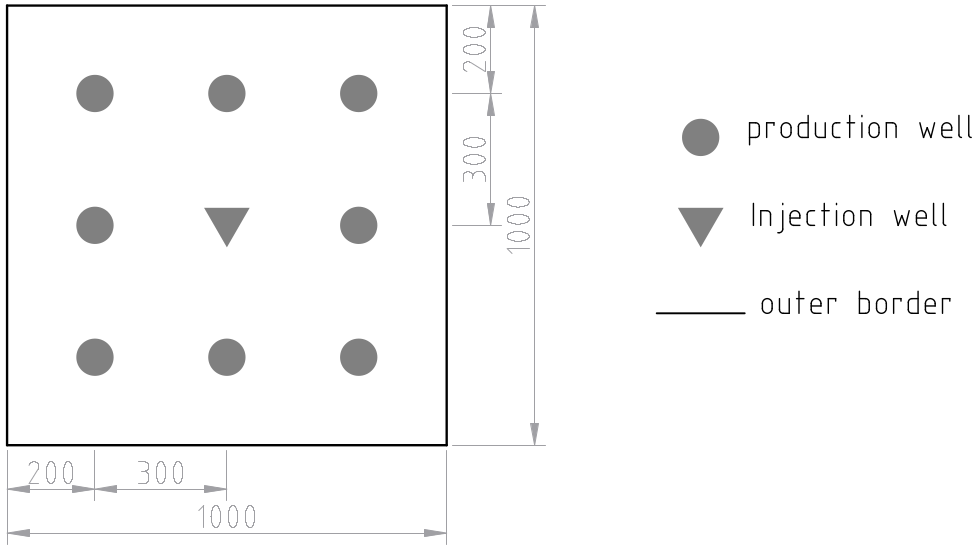
\includegraphics[height=12pc]{fig1.png}}
    \caption{Schematic representation of the computational domain.}
	\label{fig:map}
\end{figure}

The field is being developed with the help of 8 production and 1 injection wells. At the wells, the fluid flow rate was set (flow rate for producing and injection capacity for injection). The fluid flow rate for each well was set as a noisy fixed value, the noise amplitude was up to $50\%$ of the average value. The time step was 1 month. The development period is 30 years, the power circuit was “connected” along the perimeter of the computational area. To solve the problem of parametric identification, the development period was divided into 2 intervals: the history matching interval, at which the model parameters were adjusted, and the validation interval, at which the predictive characteristics of the calibrated model were evaluated. The periods were 20 and 10 years, respectively. The amount of initial data that was used when setting up the model on the history matching interval is 63 pressure values randomly selected from the entire volume of initial well pressure values, which is approximately $2.5\%$ of the available number. For the history matching interval, 1920 values of water flow in production wells were used. At the validation interval, the amount of initial data was 37 and 960 values for pressure and flow, respectively.

The direct and inverse problems were solved numerically using the control volume method, the difference grid had 441 calculated nodes, each node has its own permeability value, which is a configurable parameter.

The history matching problem is solved for 11 variants of sets of weight coefficients $(w_p, w_{q_w})$ used in the objective function {\ref{mse}}. The values of the weight coefficients in the sets were set in such a way that the condition $w_p = 1 - w_{q_w}$ was fulfilled, where $w_{q_w}$ changed from 0 to 1 with a step of 0.1. By changing the weight coefficients, the sensitivity of the objective function and its gradient to different types of input data changed. In addition, if one of the weight coefficients is equal to 0, the model is tuned to only one of the two types of input data.

Research methodology: the permeability field is set, the well operation modes (fluid flow rates) are set, the direct problem is solved, the calculated values of reservoir pressure and oil flow rate are saved and then act as actual values. Next, a perturbation is introduced into the initial permeability field, which acts as an initial approximation in solving the inverse problem. Next, the inverse problem is solved in order to restore such a permeability field in order to reproduce as accurately as possible the actual values of reservoir pressure and water flow in wells, taking into account the given weight coefficients. Further, the calibrated model performs predictive calculations, the forecast period coincides with the validation interval, which evaluates the ability of the model to reproduce the indicators of interest to us, the initial values of which did not participate in the history matching process.

The figure \ref{fig:press} shows the initial values of reservoir pressure for wells at different points in time, the vertical dotted line on this graph and on the following ones separates the intervals of history matching and validation. The figure \ref{fig:qlic} shows the dynamics of the total flow rate of fluid and water for production wells, the pictograms show the initial values, the lines show the averaging of the dynamics of the corresponding indicators.
\begin{figure} 
    \begin{minipage}[h]{0.48\linewidth}
      \center{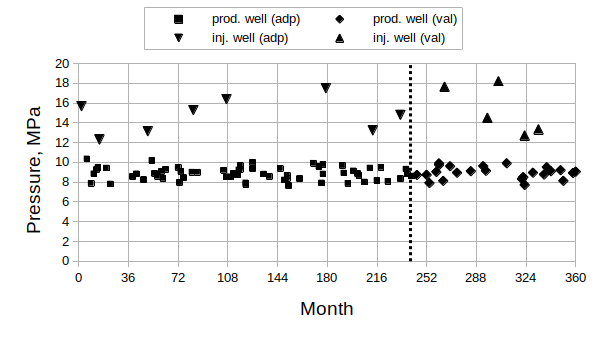
\includegraphics[height=0.60\linewidth]{fig2.png}}
      \caption{Reservoir pressure values near wells used to evaluate the accuracy of model tuning for history matching and validation intervals.}
      \label{fig:press}
    \end{minipage} \hfill
    \begin{minipage}[h]{0.48\linewidth}
      \center{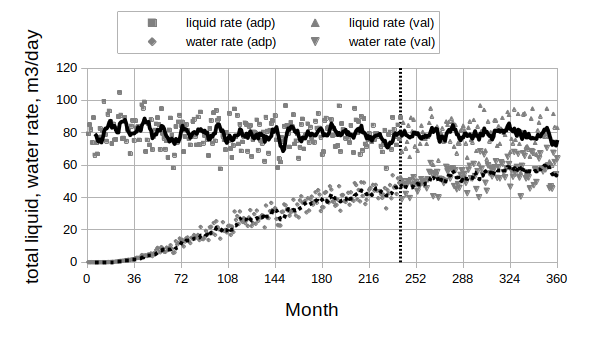
\includegraphics[height=0.60\linewidth]{fig3.png}}
      \caption{The values of the total flow rates of liquid and water for history matching and validation intervals.}
      \label{fig:qlic}
    \end{minipage} 
\end{figure}
It can be seen from the figures that the average values of the reservoir pressure and fluid flow rate are constant throughout the entire simulation period, the water flow rate gradually increases as the oil is displaced by water and the front of the water saturation jump arrives at the production wells.
The inverse problem was solved for 11 sets of weight coefficients, in which the influence of pressure data gradually increased and the influence of water flow decreased. The figure \ref{fig:wp} shows the values of the MAPE metrics and the objective function $J$ for different sets of weight coefficients. The MAPE metric is calculated for pressure indicators, water flow rates at production wells for history matching and validation intervals. In addition, the figure shows the MAPE metric for permeability, which characterizes the deviation of the restored values from the actual ones.

\begin{figure}
	\center{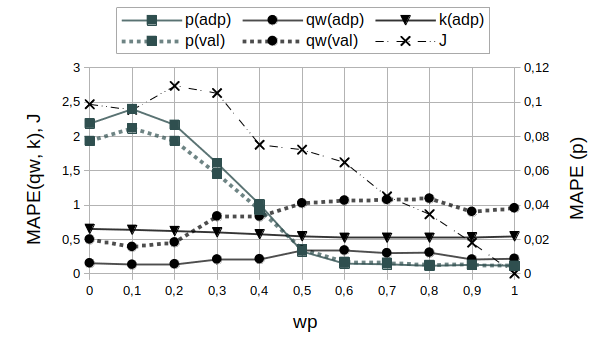
\includegraphics[height=12pc]{fig4.png}}
	\caption{MAPE metric and objective function J values for 11 sets of weight coefficients for history matching
		intervals (adp) and validation intervals (val).}
	\label{fig:wp}
\end{figure}

It can be seen from the graph that, in general, the expected inversely proportional dependence of the metric value and the corresponding weighting coefficient is observed. Similar behavior of the corresponding metrics for history matching and validation intervals is also observed. However, the sensitivity of the metric characterizing the predictive properties for the "water flow" indicator is higher than the metric of the same indicator on the history matching interval, which indicates the importance of choosing one or another history matching option in terms of predictive properties. Figure \ref{fig:wp} also shows that the nature of the change in the objective function $J$ differs from the nature of the change in the MAPE metric. Based on the graph, we can conclude that when the weight coefficient $w_p$ changes in the range from 0 to 0.3, it is most difficult for the model to satisfy the initial data. Since the main purpose of modeling is to obtain a reliable forecast, and also taking into account the nature of the dependence of metrics and their absolute values on weight coefficients, it is recommended to choose the model history matching option with the value of the weight coefficient $w_p$ = 0.1. It should also be answered that, due to the peculiarity of the solution of the inverse problem, none of the solutions reproduced the original permeability field, the deviation was more than 50\%, nevertheless, the predictive characteristics of these models are satisfactory, both for reservoir pressure and for water flow. In practice, we do not know the real permeability field, and the solution obtained for practical problems is acceptable if it has a satisfactory history setting and good predictive properties.

For the selected variant of the calibrated model and for the limiting variants ($w_p = 0$ and $w_p = 1$), let's compare the behavior of an additional integral indicator - the average water cut at the intervals of history matching and validation. The average water cut at each point in time is calculated as $wtc = \frac{\sum{q_w^i}}{\sum{q_l^i}}$. The average water cut of the produced liquid is shown in the figure \ref{fig:wtc}. Pictograms in the figure \ref{fig:wtc} show water cut values for each month, lines show averaged values for four options: the original option and 3 options of the calibrated model with the weight coefficient $w_p$ equal to 0, 0.1 and 1.

\begin{figure}
	\center{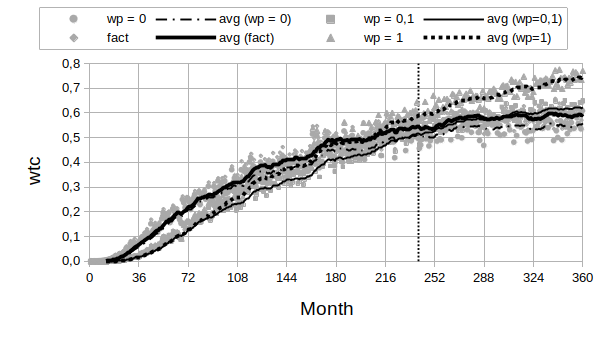
\includegraphics[height=12pc]{fig5.png}}
	\caption{Produced liquid water cut (wtc) dynamics: actual values and for 3 variants of matched model.}
	\label{fig:wtc}
\end{figure}
It can be seen from the figure that the history matching option, taking into account only reservoir pressure $(w_p=1)$, differs markedly from the original option both at the stage of history matching and at the validation interval. The history matching option, which takes into account only water flow rates $(w_p=0)$, differs to a lesser extent from the original option, this is due to the fact that the flow rate of phases in wells depends both directly on the formation pressure and on the structure of filtration flows in the interwell space, which in turn depends on reservoir pressure. This can also be seen from the \ref{dq_du} equation, where the derivative of water flow from permeability depends on the derivative of pressure from permeability. From the point of view of forecasting, the best history matching option is that which takes into account pressure and water flow in a complex way, the reduced weighting coefficient $(w_p=1)$ is explained by the fact that the dependence on reservoir pressure, as mentioned earlier, is included in the term of the objective function responsible for water flow and is indirectly taken into account. Nevertheless, the presence of the term responsible for reservoir pressure is important during the dry period of operation, when the front of the water saturation jump has not yet reached the production wells. Thus, the use of the sum as the objective function allows more complete use of all available information throughout the entire modeling period.

\section{CONCLUSIONS}

As a result of the study, it was shown that the accuracy of solving the inverse problem depends on the choice of weight coefficients that characterize the degree of influence on the setting of a certain type of data. The use of a combination of initial data makes it possible to increase the degree of regularization of the problem. The accuracy of the model for the history matching and validation periods depends on the proportions of the weights chosen. The dependence of the accuracy of tuning and forecasting for an individual indicator is not linear on the corresponding weight coefficient. The dependence is characterized by the presence of minima and maxima, which indicates that the degree of consideration of different indicators affect the tuning process and can help to find the most accurate solution. In view of the peculiarities of the methodology for solving inverse problems in the optimization formulation, which consists in minimizing one function that includes heterogeneous data, it is advisable to analyze other metrics that allow us to evaluate the accuracy of tuning and forecasting on the other hand. Given the availability of a set of calibrated models, third-party metrics will allow you to choose the most appropriate model in terms of the requirements for it.


\section{FUNDING}
The research was carried out within the state assignment of Ministry of Science and Higher Education of the Russian Federation (project No. 121030500156-6).

%
% The Bibliography
%
\begin{thebibliography}{99}
	
\bibitem{mus} E.N.Musakaev, S.P.Rodionov, D.Y.Legostaev, V.P.Kosyakov, "Parameter identification for sector filtration model of an oil reservoir with complex structure" // AIP Conference Proceedings 2125,030113 2019;

\bibitem{kos} V. P. Kosyakov. "Structural and Parametric Identification of an Aquifer Model for an Oil Reservoir". Lobachevskii J Math. 2020. V. 41, P. 1242-1247.

\bibitem{bas} K. S. Basniev, N. M. Dmitriev, R. D. Kanevskaya, V. M. Maksimov. \textit{Underground hydromechanics}. M.-Izhevsk: Institute for Computer Research, 2006. [in Russian]

\bibitem{azi} H. Aziz, E. Settari. \textit{Mathematical modeling of reservoir systems}.  M.-Izhevsk: Institute for Computer Research, 2004. [in Russian]

\bibitem{opt} V.P.Kosyakov, S.P.Rodionov "Optimal control of wells on the basis of two-phase filtration equations". Proceedings of MIPT. 2016. V. 8, N 3. P. 79-90.

\bibitem{leg} V. P. Kosyakov,  D. Yu. Legostaev. "Using elements of machine learning to
solve the inverse problem of reconstructing the hydraulic conductivity feld for a fltration
problem". Tyumen State University Herald. Physical and Mathematical Modeling. Oil, Gas,
Energy, V. 8, N 2 (30), P. 129-149.


\end{thebibliography}

\end{document}